\usetikzlibrary{positioning}

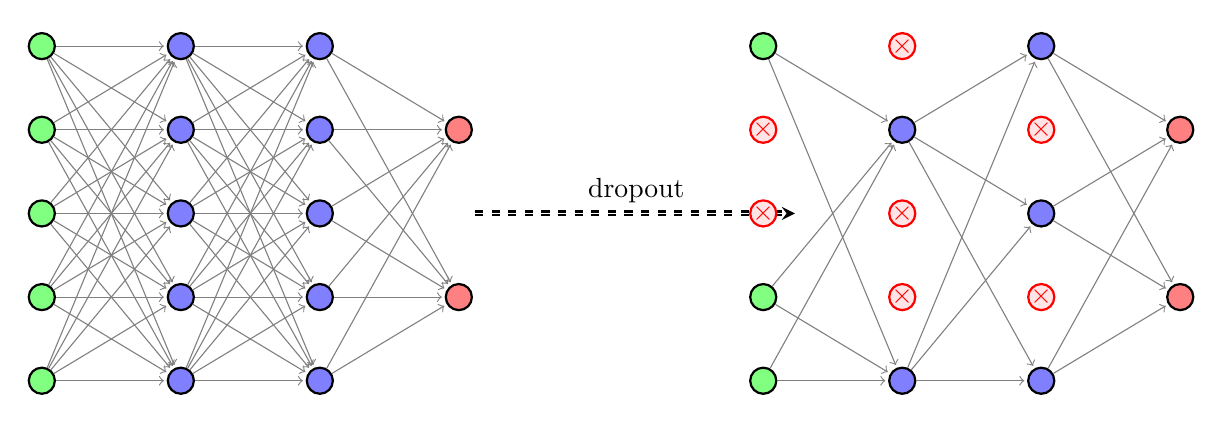
\begin{tikzpicture}[shorten >=1pt,->,draw=black!50]
	\tikzstyle{every pin edge}=[<-,shorten <=0pt]

	\node[circle, draw=black!100, thick, fill=green!50] (i1) {};
	\node[circle, draw=black!100, thick, fill=green!50, above=2em of i1] (i2) {};
	\node[circle, draw=black!100, thick, fill=green!50, above=2em of i2] (i3) {};
	\node[circle, draw=black!100, thick, fill=green!50, below=2em of i1] (i4) {};
	\node[circle, draw=black!100, thick, fill=green!50, below=2em of i4] (i5) {};
	
	\node[circle, draw=black!100, thick, fill=blue!50, right=4em of i1] (h1) {};
	\node[circle, draw=black!100, thick, fill=blue!50, right=4em of i2] (h2) {};
	\node[circle, draw=black!100, thick, fill=blue!50, right=4em of i3] (h3) {};
	\node[circle, draw=black!100, thick, fill=blue!50, right=4em of i4] (h4) {};
	\node[circle, draw=black!100, thick, fill=blue!50, right=4em of i5] (h5) {};
	
	\node[circle, draw=black!100, thick, fill=blue!50, right=4em of h1] (hh1) {};
	\node[circle, draw=black!100, thick, fill=blue!50, right=4em of h2] (hh2) {};
	\node[circle, draw=black!100, thick, fill=blue!50, right=4em of h3] (hh3) {};
	\node[circle, draw=black!100, thick, fill=blue!50, right=4em of h4] (hh4) {};
	\node[circle, draw=black!100, thick, fill=blue!50, right=4em of h5] (hh5) {};
	
	\node[circle, draw=black!100, thick, fill=red!50, right=4em of hh2] (o1) {};
	\node[circle, draw=black!100, thick, fill=red!50, right=4em of hh4] (o2) {};
	
	\path (i1) edge (h1);
	\path (i1) edge (h2);
	\path (i1) edge (h3);
	\path (i1) edge (h4);
	\path (i1) edge (h5);
	\path (i2) edge (h1);
	\path (i2) edge (h2);
	\path (i2) edge (h3);
	\path (i2) edge (h4);
	\path (i2) edge (h5);
	\path (i3) edge (h1);
	\path (i3) edge (h2);
	\path (i3) edge (h3);
	\path (i3) edge (h4);
	\path (i3) edge (h5);
	\path (i4) edge (h1);
	\path (i4) edge (h2);
	\path (i4) edge (h3);
	\path (i4) edge (h4);
	\path (i4) edge (h5);
	\path (i5) edge (h1);
	\path (i5) edge (h2);
	\path (i5) edge (h3);
	\path (i5) edge (h4);
	\path (i5) edge (h5);
	
	\path (h1) edge (hh1);
	\path (h1) edge (hh2);
	\path (h1) edge (hh3);
	\path (h1) edge (hh4);
	\path (h1) edge (hh5);
	\path (h2) edge (hh1);
	\path (h2) edge (hh2);
	\path (h2) edge (hh3);
	\path (h2) edge (hh4);
	\path (h2) edge (hh5);
	\path (h3) edge (hh1);
	\path (h3) edge (hh2);
	\path (h3) edge (hh3);
	\path (h3) edge (hh4);
	\path (h3) edge (hh5);
	\path (h4) edge (hh1);
	\path (h4) edge (hh2);
	\path (h4) edge (hh3);
	\path (h4) edge (hh4);
	\path (h4) edge (hh5);
	\path (h5) edge (hh1);
	\path (h5) edge (hh2);
	\path (h5) edge (hh3);
	\path (h5) edge (hh4);
	\path (h5) edge (hh5);
	
	
	\path (hh1) edge (o1);
	\path (hh1) edge (o2);
	\path (hh2) edge (o1);
	\path (hh2) edge (o2);
	\path (hh3) edge (o1);
	\path (hh3) edge (o2);
	\path (hh4) edge (o1);
	\path (hh4) edge (o2);
	\path (hh5) edge (o1);
	\path (hh5) edge (o2);
	
	\draw[-stealth, double, dashed, draw=black!100, thick] (5.5,0) -- node[above] {dropout} (9.6, 0);
	
	
	%%% BOUNDARY %%%
	
	\node[circle, draw, thick, red, fill=red!10, right=15em of hh1] (i1) {};
	\node[circle, draw, thick, red, fill=red!10, above=2em of i1] (i2) {};
	\node[circle, draw=black!100, thick, fill=green!50, above=2em of i2] (i3) {};
	\node[circle, draw=black!100, thick, fill=green!50, below=2em of i1] (i4) {};
	\node[circle, draw=black!100, thick, fill=green!50, below=2em of i4] (i5) {};
	
	\node[red] (icr) at (i1) {$\mathlarger{\mathlarger{\mathlarger{\mathlarger{\mathlarger{\bm{\times}}}}}}$};
	\node[red] (icr) at (i2) {$\mathlarger{\mathlarger{\mathlarger{\mathlarger{\mathlarger{\bm{\times}}}}}}$};
	
	\node[circle, draw, thick, red, fill=red!10, right=4em of i1] (h1) {};
	\node[circle, draw=black!100, thick, fill=blue!50, right=4em of i2] (h2) {};
	\node[circle, draw, thick, red, fill=red!10, right=4em of i3] (h3) {};
	\node[circle, draw, thick, red, fill=red!10, right=4em of i4] (h4) {};
	\node[circle, draw=black!100, thick, fill=blue!50, right=4em of i5] (h5) {};
	
	\node[red] (icr) at (h1) {$\mathlarger{\mathlarger{\mathlarger{\mathlarger{\mathlarger{\bm{\times}}}}}}$};
	\node[red] (icr) at (h3) {$\mathlarger{\mathlarger{\mathlarger{\mathlarger{\mathlarger{\bm{\times}}}}}}$};
	\node[red] (icr) at (h4) {$\mathlarger{\mathlarger{\mathlarger{\mathlarger{\mathlarger{\bm{\times}}}}}}$};
	
	\node[circle, draw=black!100, thick, fill=blue!50, right=4em of h1] (hh1) {};
	\node[circle, draw, thick, red, fill=red!10, right=4em of h2] (hh2) {};
	\node[circle, draw=black!100, thick, fill=blue!50, right=4em of h3] (hh3) {};
	\node[circle, draw, thick, red, fill=red!10, right=4em of h4] (hh4) {};
	\node[circle, draw=black!100, thick, fill=blue!50, right=4em of h5] (hh5) {};
	
	\node[red] (icr) at (hh2) {$\mathlarger{\mathlarger{\mathlarger{\mathlarger{\mathlarger{\bm{\times}}}}}}$};
	\node[red] (icr) at (hh4) {$\mathlarger{\mathlarger{\mathlarger{\mathlarger{\mathlarger{\bm{\times}}}}}}$};
	
	\node[circle, draw=black!100, thick, fill=red!50, right=4em of hh2] (o1) {};
	\node[circle, draw=black!100, thick, fill=red!50, right=4em of hh4] (o2) {};
	
	\path (i3) edge (h2);
	\path (i3) edge (h5);
	\path (i4) edge (h2);
	\path (i4) edge (h5);
	\path (i5) edge (h2);
	\path (i5) edge (h5);
	
	\path (h2) edge (hh1);
	\path (h2) edge (hh3);
	\path (h2) edge (hh5);
	\path (h5) edge (hh1);
	\path (h5) edge (hh3);
	\path (h5) edge (hh5);
	
	\path (hh1) edge (o1);
	\path (hh1) edge (o2);
	\path (hh3) edge (o1);
	\path (hh3) edge (o2);
	\path (hh5) edge (o1);
	\path (hh5) edge (o2);

\end{tikzpicture}